%% analyse.tex
%% $Id: analyse.tex 28 2007-01-18 16:31:32Z bless $

\chapter{Schlafanalyse}
\label{ch:sa}
Zur Analyse eines respiratorischen Ereignisses findet im Zuge dieser Bachelorarbeit eine Nutzerstudie statt, um einen Datensatz zu erstellen, welcher daraufhin analysiert werden kann. Im Folgenden wird erläutert, welche Geräte verwendet werden und wie diese gesammelten Informationen zusammengetragen werden, damit der entstehende Datensatz in einem strukturierten Zustand vorliegt.

\section{Earable Plattform}
\label{ch:sa:ep}
Zur Erfassung der Daten werden eSense-Earpods der Firma ``Nokia Bell Labs Cambridge'' verwendet.	
Die Earpods beinhalten zwei Mikrofone und einen Lautsprecher, welche beide über Bluetooth angebunden werden können.
Pro Earpod ist ein Mikrofon verbaut.
Des weiteren ist das für diese Bachelorarbeit interessanteste Element, eine 6-Achsen IMU (Inertial Motion Unit) Teil der Earpods.
Eine IMU ist eine inertiale Messeinheit, womit Gyroskop- und Beschleunigungsdaten aufgezeichnet und mittels BLE (Bluetooth Low Energy) auf das Smartphone übertragen werden können. 
Es handelt sich um einen 3-Achsen Beschleunigungssensor, sowie ein 3-Achsen Gyroskop.
Die IMU ist lediglich im linken Earpod verbaut.
Die Messrate dieser Sensoren ist variabel einstellbar und wurde im Folgenden auf $50 \si{\hertz}$ festgelegt.
Die IMU ist ebenfalls konfigurierbar und wurde nicht verändert. 
Dieser Messbereich ist beim Beschleunigungssensor $\pm 4g$ und beim Gyroskop $\pm 500deg/s$.
Die Messdaten der IMU sind bereits gefiltert, wenn sie per BLE übertragen werden.
Hier wurde die Konfiguration ebenfalls auf den Standardwerten belassen, was bedeutet, dass ein Tiefpassfilter mit einer Bandbreite von $5\si{\hertz}$ auf die Beschleunigungs- und Gyroskopdaten angewandt wird.

\begin{figure}[ht]
    \centering
    \begin{subfigure}{.49\textwidth}
      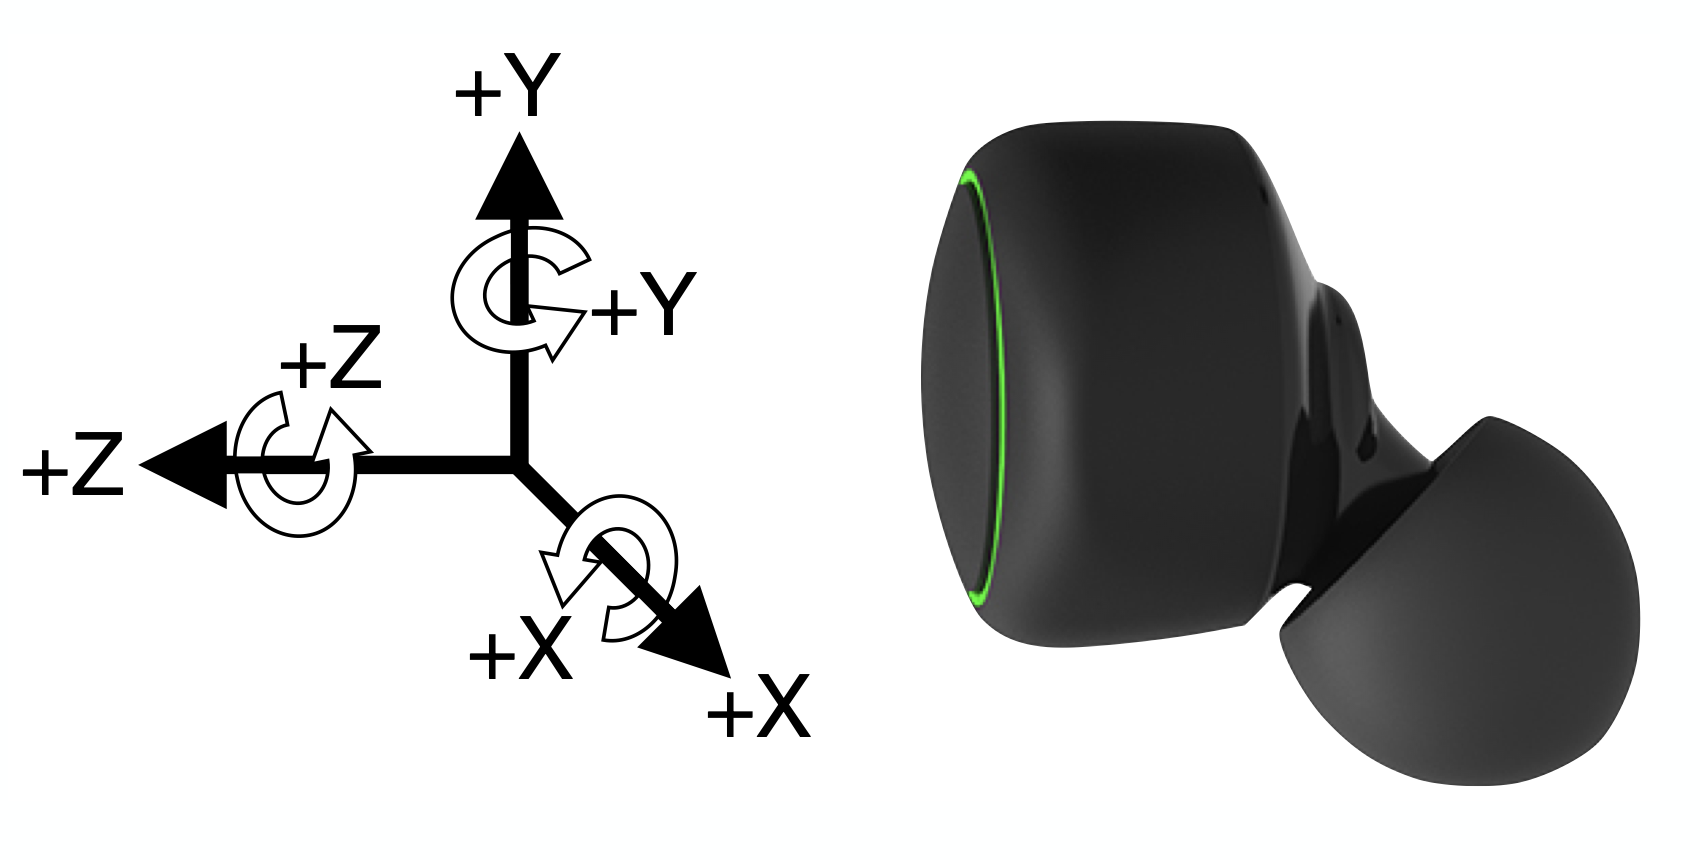
\includegraphics[width=1\textwidth]{eSense/eSense_earpod_rotation}
      \caption{Achsen der IMU in den eSense Earpods}
      \label{analysis:eSense:rotation}
    \end{subfigure}
    \begin{subfigure}{.49\textwidth}
      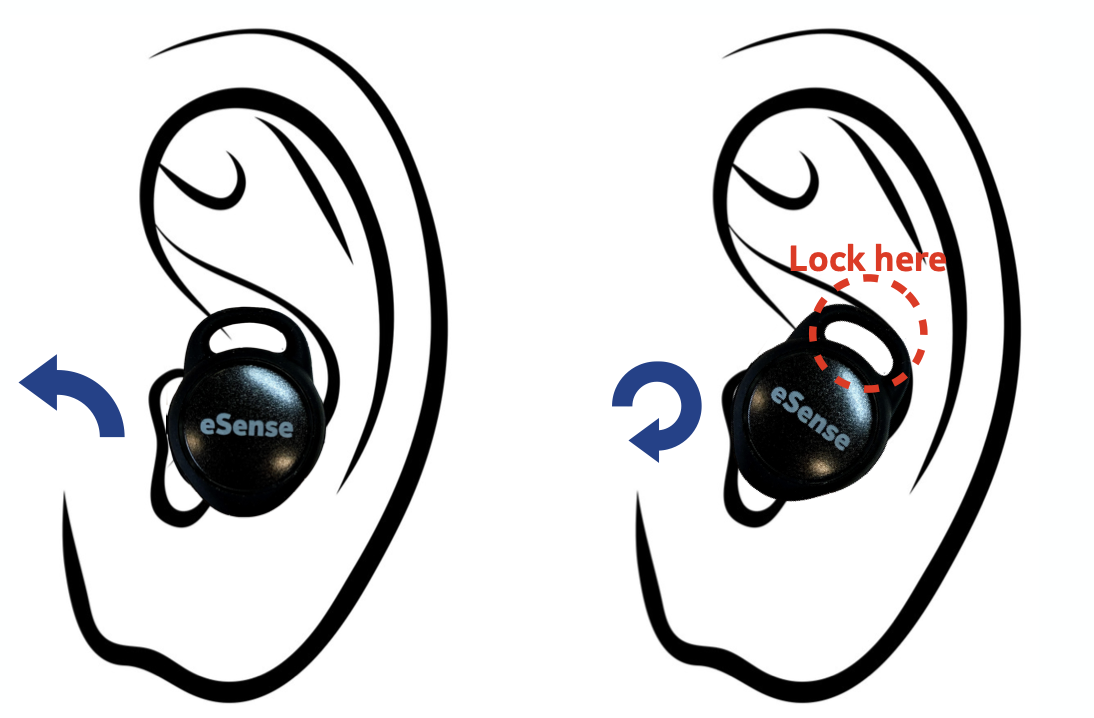
\includegraphics[width=0.9\textwidth]{eSense/eSense_how_to_wear}
      \caption{Trageposition der eSense Earpods}
      \label{analysis:eSense:how_to_wear}
    \end{subfigure}
    \label{analysis:eSense:images}
  \end{figure}

\subsection{Was wird aufgezeichnet?}
\label{ch:sa:ep:what_to_record}
Zur vollständigen Aufzeichnung eines Datensatzes werden die Daten der IMU, in einer Datenbank abgespeichert.
Insgesamt werden hierbei pro empfangene Dateneinheit 6 Werte persistiert, die \textit{x, y} und \textit{z} Richtung des Beschleunigungs- und Gyroskopsensors. 
Des weiteren wird die aktuelle Zeit, die aktuell auszuführende Aktion des Studienablaufs und die Information, ob die LED des Smartphones an oder aus ist, zu jeder empfangenen Dateneinheit hinzugefügt.
Das Mikrofon wird ebenfalls aufgezeichnet und nach der Messsung abgespeichert.
Vor dem Beginn einer Messung wird der Studienteilnehmer gebeten, ein paar Zusatzinformationen (siehe Kapitel \ref{ch:sa:additionalUserStudiesInformation}) anzugeben.
Diese werden vor dem Start der Messung am Smartphone ausgefüllt und ebenfalls in der Datenbank gespeichert.

\subsection{Datenexport}
\label{ch:sa:ep:export}
Zur weiteren Verarbeitung werden die Daten, nachdem sie von der App lokal in einer Datenbank gespeichert werden, exportiert. 
Zuerst werden die Datenbankeinträge der aktuellen Messung als \textit{csv}-Datei exportiert und in einem temporären Ordner abgespeichert.
Hierbei werden die Gyroskop- und Beschleunigungsdaten separat exportiert und es entstehen 2 \textit{csv}-Dateien (\glqq \textit{GyroData\_\$ID\$.csv}\grqq, \glqq \textit{ACCData\_\$ID\$.csv}\grqq).
Das Mikrofon-Signal wird nach der Messung als \textit{m4a}-Datei im temporären Ordner abgelegt.
Die Zusatzinformationen, welche über den Studienteilnehmer hinterlegt wurden, werden als \textit{csv}-Datei (\glqq \textit{UserStudyPersonDetails\_\$ID\$.csv}\grqq) ebenfalls in den temporären Ordner persistiert.
Alle Dateien des temporären Ordners werden in einer zip-Datei verpackt und können über den Share-Screen von Apple über verschiedene Wege geteilt werden.

\section{Polysomnographie-Systeme}
\label{ch:sa:psg}
Als Referenz zu den eSense-Earpods wird ein Polysomnographie-System (PSG-System) verwendet. 
Das Gerät SOMNOscreen{\texttrademark} plus bietet alle nötigen Sensoren und findet in der Wissenschaft Anerkennung.
Ein solches System zeichnet Messungen für physiologische Funktionen des Körpers während des Schlafs auf und kann somit mögliche Schlafstörungen diagnostizieren.
Im Gegensatz zur Polygraphie kann die Polysomnographie explizit zwischen obstruktiver und zentraler Apnoe unterscheiden \cite{croenleinSchlafmedizin1x1Praxisorientiertes2017}.
Es werden kontinuierlich verschiedene Körperfunktionen überwacht, wodurch nach einer Messung ein umfangreiches und individuelles Schlafprofil erstellt werden kann.

\begin{figure}[ht]
    \centering
    \begin{subfigure}{.4\textwidth}
        \begin{center}
            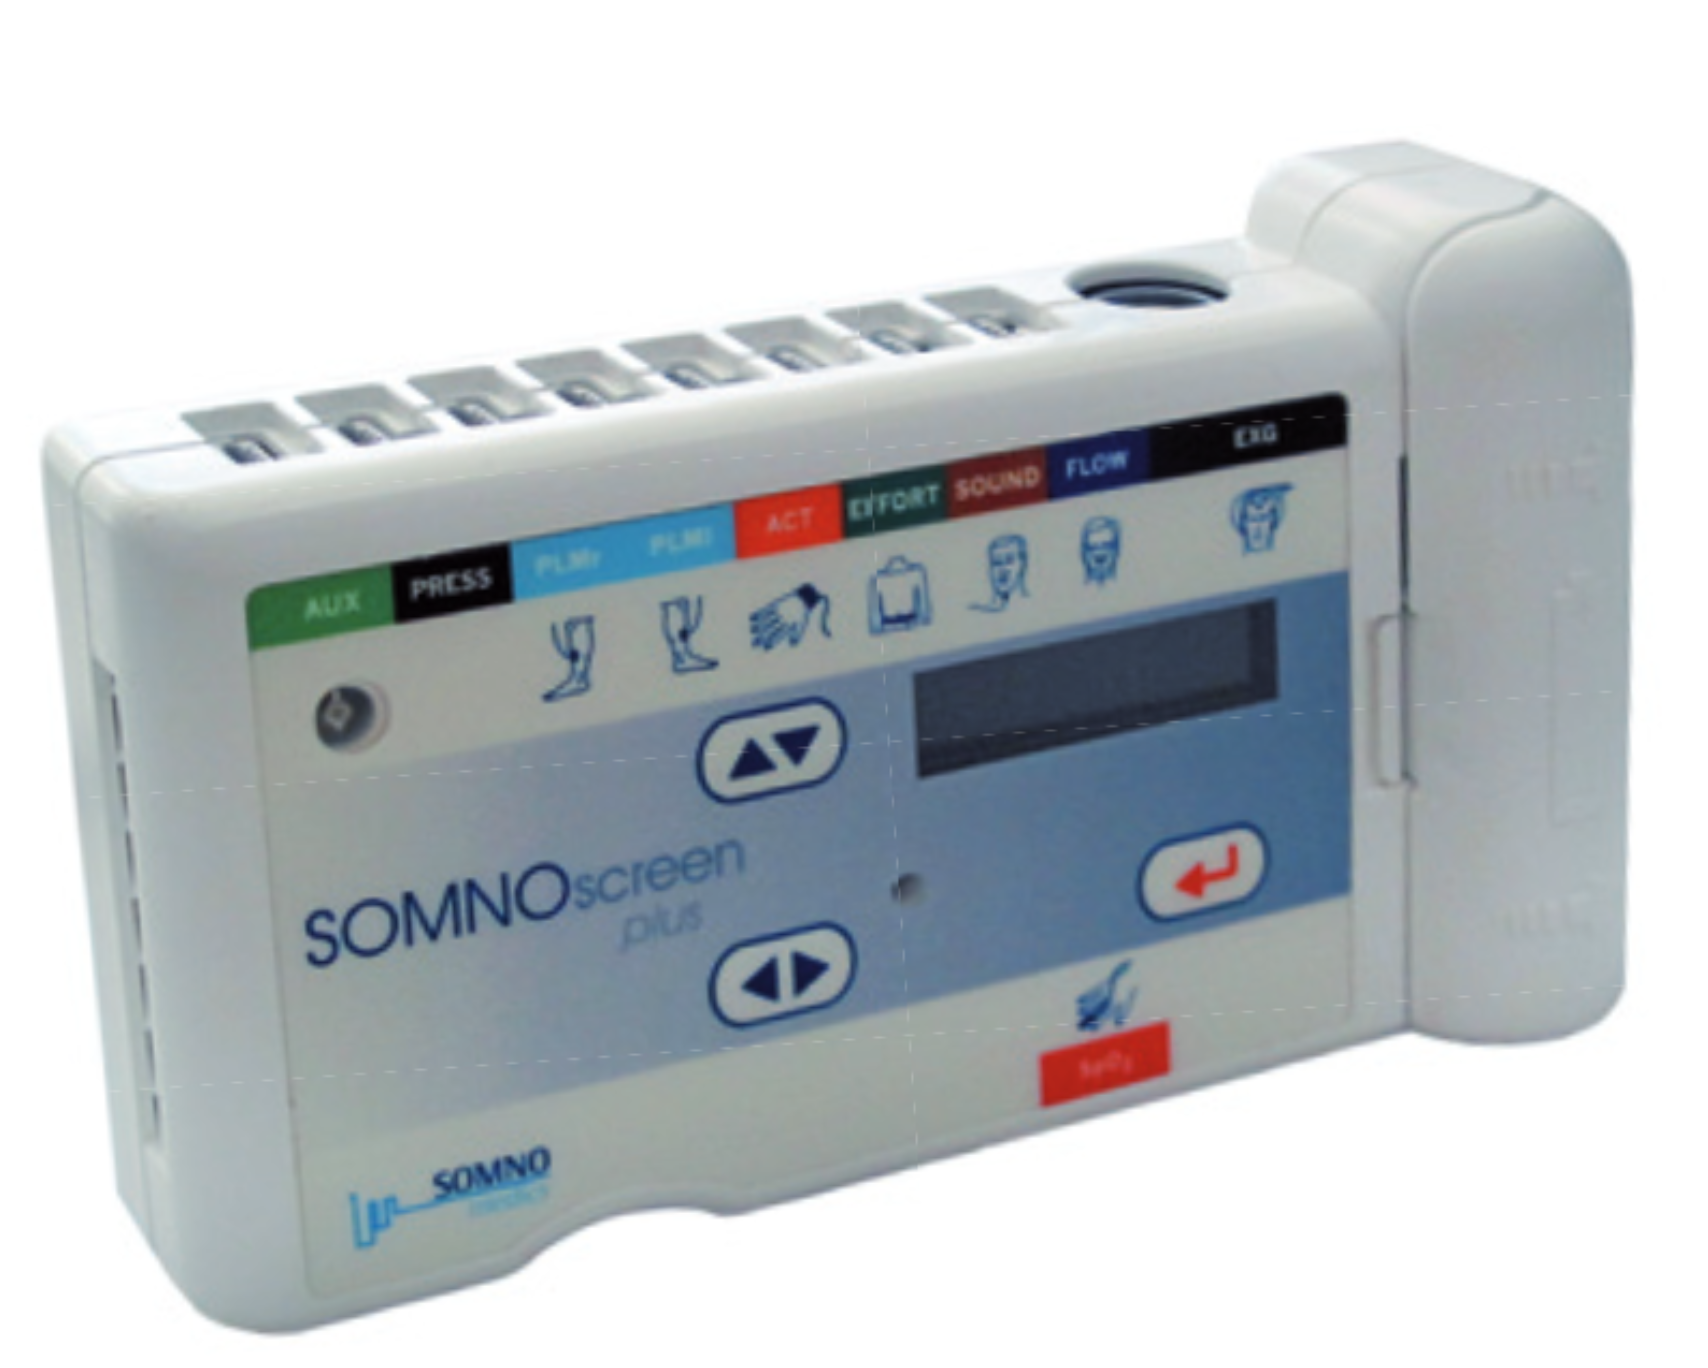
\includegraphics[width=1\textwidth]{study/psg_system_picture}
        \end{center}
        \caption{{SOMNOscreen \texttrademark} plus}
    \end{subfigure}
    \begin{subfigure}{.58\textwidth}
        \begin{center}
            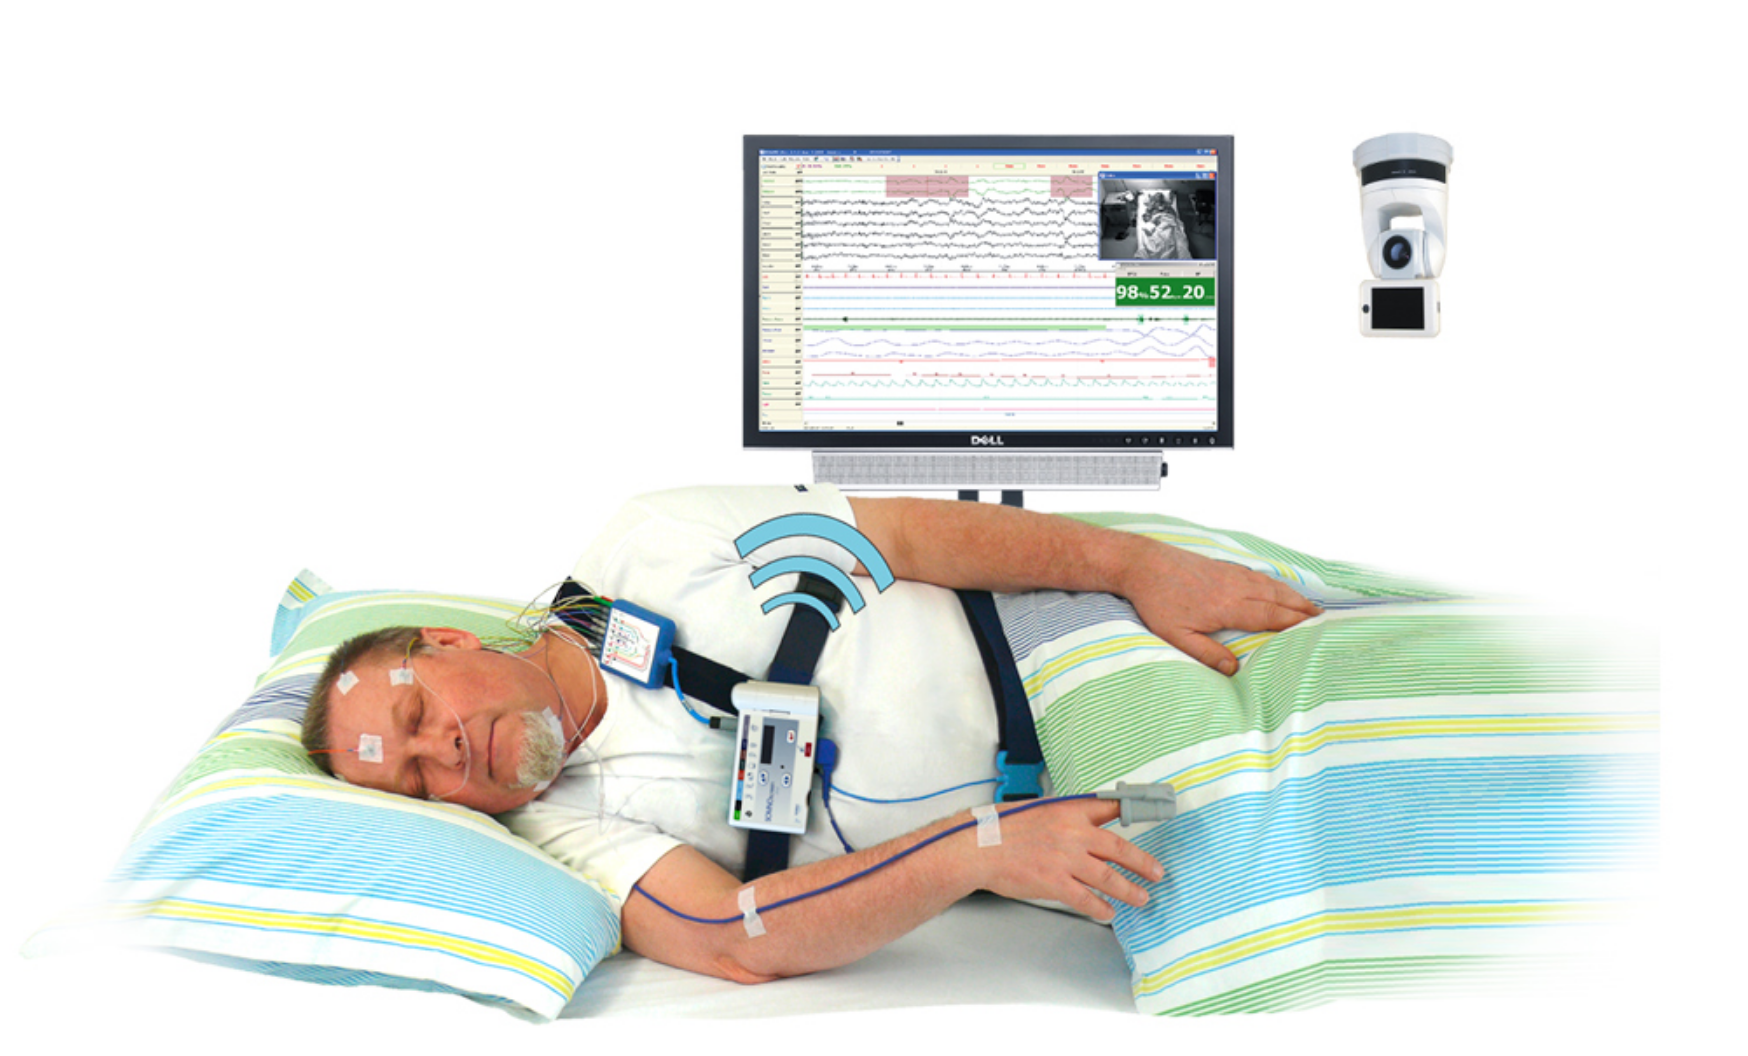
\includegraphics[width=0.92\textwidth]{study/psg_system_flow.png}
        \end{center}
        \caption{Polysomnographie: Ablauf}
    \end{subfigure}
    \caption{PSG-System im Einsatz und die visuelle Darstellung\protect\footnotemark}
    \label{analysis:psg:picture}
  \end{figure}
  \footnotetext{siehe Quelle: \cite{SomnomedicsSomnoscreenBroschure}}


Das PSG-System zeichnet während der Studie ebenfalls Daten auf und soll die Resultate, welche durch die eSense-Earpods gesammelt und analysiert werden, verifizieren. Somit dienen die Daten, welche durch das PSG-System gesammelt werden, als \glqq Ground-Truth\grqq.

Mittels der {\glqq DOMINO Schlafdiagnostik\grqq} Software kann eine Montage erstellt werden. 
Eine Montage ist eine Konfiguration, bei der man festlegen kann, welche Sensoren gemessen und persistiert werden sollen. Zudem kann man die Abtastrate in $\si{\hertz}$ festlegen.
In der Abbildung \ref{implementation:study:measurement_example} ist eine Person zu sehen, welche alle für die Studie relevanten Sensoren trägt.
Im Folgenden werden alle Sensoren aufgelistet, welche für die Studie aufgezeichnet wurden und somit die Montage darstellen.

\begin{itemize}
    \item \textbf{Bauchsignal (\texttt{abdomen}) ($32 \si{\hertz}$)}: gibt die Veränderung des Volumens am Bauch an.
    \item \textbf{Lichtsignal (\texttt{light}) ($128 \si{\hertz}$)}: Misst das Umgebungslicht, was verwendet wird, um die Signale vom PSG-System und den eSense-Earpods zu synchronisieren.
    \item \textbf{Drucksignal (\texttt{flow}) ($256 \si{\hertz}$)}: Hier wird der Druck gemessen, der durch die Nase kommt. Der Sensor ist direkt an der Nase befestigt.
    \item \textbf{Bewegungssignal (\texttt{movement}) ($32 \si{\hertz}$)}: Es misst die Bewegung anhand von Beschleunigungsdaten.
    \item \textbf{Sauerstoffsättigung (\texttt{pleth}) ($128 \si{\hertz}$)}: Sie gibt die Sauerstoffsättigung im Blut an.
    \item \textbf{Pulssignal (\texttt{pulse}) ($32 \si{\hertz}$)}: Gibt den Puls, gemessen am Finger des Patienten, an.
    \item \textbf{Schnarchmikrofonsignal (\texttt{schnarch}) ($256 \si{\hertz}$)}: Dieser Sensor wird am Kehlkopf befestigt und misst das Schnarchen.
    \item \textbf{Sauerstoffgehalt (\texttt{spo2}) ($32 \si{\hertz}$)}: Dieser wird anhand einer manschettenfreien kontinuierlichen Blutdruckmessung ermittelt.
    \item \textbf{Brustkorbsignal (\texttt{thorax}) ($32 \si{\hertz}$)}: Es gibt die Veränderung des Volumens am Brustkorb an.
    \item \textbf{Brustkorb \& Bauchsignal (\texttt{thoraxabdomen}) ($32 \si{\hertz}$)}: kombiniertes Signal von Brust- und Bauchsignal
    \item \textbf{EDF Informationen (\texttt{edfAnnotations}) ($60 \si{\hertz}$)}: Sie enthalten Anmerkungen als \textit{char}, z.B die Startzeit der Messung.
\end{itemize}

\subsection{Datenexport}
\label{ch:sa:psg:export}

Im PSG-System befindet sich eine CF-Karte (\textit{Compact-Flash}). Diese kann mihilfe der vom PSG-System bereitgestellten {\glqq DOMINO Schlafdiagnostik\grqq} Software ausgelesen werden.
Die Software stellt eine Darstellung bereit, womit man die Signale untereinander in einer zeitlich synchronisierten Ansicht betrachten kann. Die aufgezeichneten Signale können als \textit{edf}-Datei exportiert werden.
Mittels Python kann man \textit{edf}-Dateien auslesen und weiterverarbeiten.
Pro Studie wurden alle 3 Positionsabläufe in einem einzigen Messvorgang aufgezeichnet. Somit müssen die 3 Einzelmessugen aus der \textit{edf}-Datei herausgezogen werden.
Für weitere Details wird auf Kapitel \ref{ch:Implementierung:way_to_pipeline} verwiesen.

\section{Kamera}
\label{ch:sa:camera}
Während der Studie wurde zur vollständigen Erstellung eines Datensatzes eine Kamera mit Stativ aufgestellt, welche den Kopf des Studienteilnehmers fokussiert. 
Somit können eventuelle Unklarheiten im Datensatz, wie zum Beispiel ein Husten der Person, genau deklariert werden. 
Die verwendete Kamera ist eine \glqq Canon EOS 6D Mk II\grqq.
Die Aufnahme wurde in $1080p$ mit einer Abtastrate von $50fps$ aufgenommen.
Die Daten wurden nicht in die Klassifikation mit eingebunden und sind nur dazu gedacht, Unklarheiten auszuräumen.

\section{Datensynchronisation}
\label{ch:sa:data_synchronisation}
Um sicherzugehen, dass das PSG-System, sowie die Daten der eSense-Earpods zeitlich exakt übereinstimmt, wurden mit der App kurze Lichtblitze gesendet ($20 \si{\ms}$).
Mit einem 3D-Drucker wurde eine Vorrichtung angefertigt, welche das Smartphone auf das PSG-System platziert, sodass die LED des Smartphones direkt auf den Lichtsensor zeigt (siehe Abbildung \ref{study:3d_print}).

\begin{figure}[ht]
    \centering
    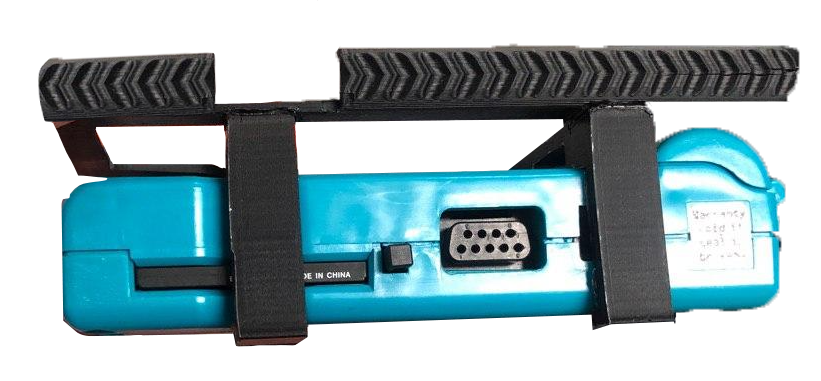
\includegraphics[width=0.7\textwidth]{study/3d_print_4}
    \caption{3D-Druck, welcher die LED des Smartphones auf den Lichtsensor zeigen lässt}
    \label{study:3d_print}
  \end{figure}

Die Lichtblitze lösen nach jeder Aktionsänderung aus, die der Studienteilnehmer erhält. 
Den genauen Ablauf kann man der Abbildung \ref{fig_study_flow} entnehmen.
Die Lichtblitze der Messung können nun mit den Lichtblitzen der eSense-Daten synchronisiert werden (siehe Kapitel \ref{ch:Implementierung:data_sync}).

\section{Zusatzinformationen der Nutzer}
\label{ch:sa:additionalUserStudiesInformation}
Vor dem Start der Datenaufzeichnung wurden Informationen über die Aufzeichnung und über die Teilnehmer gesammelt. 
Dies soll lediglich dazu dienen, spätere Unklarheiten im Datensatz erklären zu können.
Es werden Informationen zum Körper der Personen abgefragt (Alter, Größe, Gewicht, Geschlecht, Schlafrhythmus), zum Earpodaufsatz, zur Matratzenart, sowie zu den Maßen des jeweiligen Ohrs.

